\chapter{Architecture}
\label{chapter:architecture}

\section{Introduction}
\label{section:introduction}
In this chapter, the architecture of the learning environment will be regarded more closely. First of all, the central programming concept will be presented. Later, the general structure of the environment will be explained as well as the different parts.  Besides this, the goal is that an explanation for the design choices can be provided and a technical understanding for future additions to the program can be provided.

\section{Concept of Components}
\label{section:components}

In Vue.js, one can create program parts called components that can be reused in any part of the program \cite{Vue}. This can be highly useful, since many functions are used multiple times in a program, even with similar style and structure. Components can be used as a whole page (then called \nameref{section:views}) or as a part of a page or another component. For example, in every game a \nameref{subsection:buttonbar} for in-game functions is required. Instead of copying all the code for this function into every single game, one can create a component and then access it with a simple keyword. This improves not only the efficiency of the programmer, but also facilitates updates and keeps the code easy to read and understand. 

The project can be split up into components. The largest component is called App.vue. This component contains all the elements of the web application and will be rewritten and injected into the HTML file that then displays the website. App.vue contains all other components that are part of the learning environment. Each component contained in App.vue is called a child of the latter component, or even a grandchild, if it is nested within another component that is in App.vue.


\section{Layout}
\label{section:layout}
As presented in the previous section, the design concept of the learning environment requires the build-up and layout of any page of the program to be as simple and intuitive as possible. In order to cope with these requirements, the layout of the page contains of two main building blocks. The first block is the navigation bar on top of every page and the second is the routing container that displays the currently selected page. In the following, both integral parts of the platform are analysed more closely and their interconnection will be elaborated.


\subsection{Navigation Bar}
The navigation bar is placed in the top right corner of the page. For each page, it individually displays all the necessary functions that help to navigate or perform a special action. Here, one can find all buttons that are not directly involved with the task itself. All other buttons can be found in the game button bar. The navigation bar contains a function to return to the home screen, browse the about page, a print, full screen, and language switch function.

\subsubsection{Home Button}
The home button appears whenever the user is visiting another page than the home screen. This enables one to return to the main menu independent of which page has been loaded.


\begin{figure}[h]
    \centering
    
\includegraphics[width=0.2 \columnwidth]{figures/home.png}
    \caption{The Home Button} 
    \label{fig:next} 
\end{figure}

\subsubsection{Print Button}
The print button, represented by the printer icon, allows the user to print out a page. The page is formatted such that it can be printed in a better way. The program automatically renders all the relevant components in landscape mode and without the button menu and the navigation bar that are not needed on a printed page. Please note that on most computers, the print button does only print in landscape mode, as there is not enough space in portrait mode to print the whole page correctly. An example can be found in figure \ref{fig:printex}.

\begin{figure}[h]
    \centering
    
\includegraphics[width=0.2 \columnwidth]{figures/print.png}
    \caption{The Print Button} 
    \label{fig:next} 
\end{figure}

\begin{figure}[h]
    \centering
    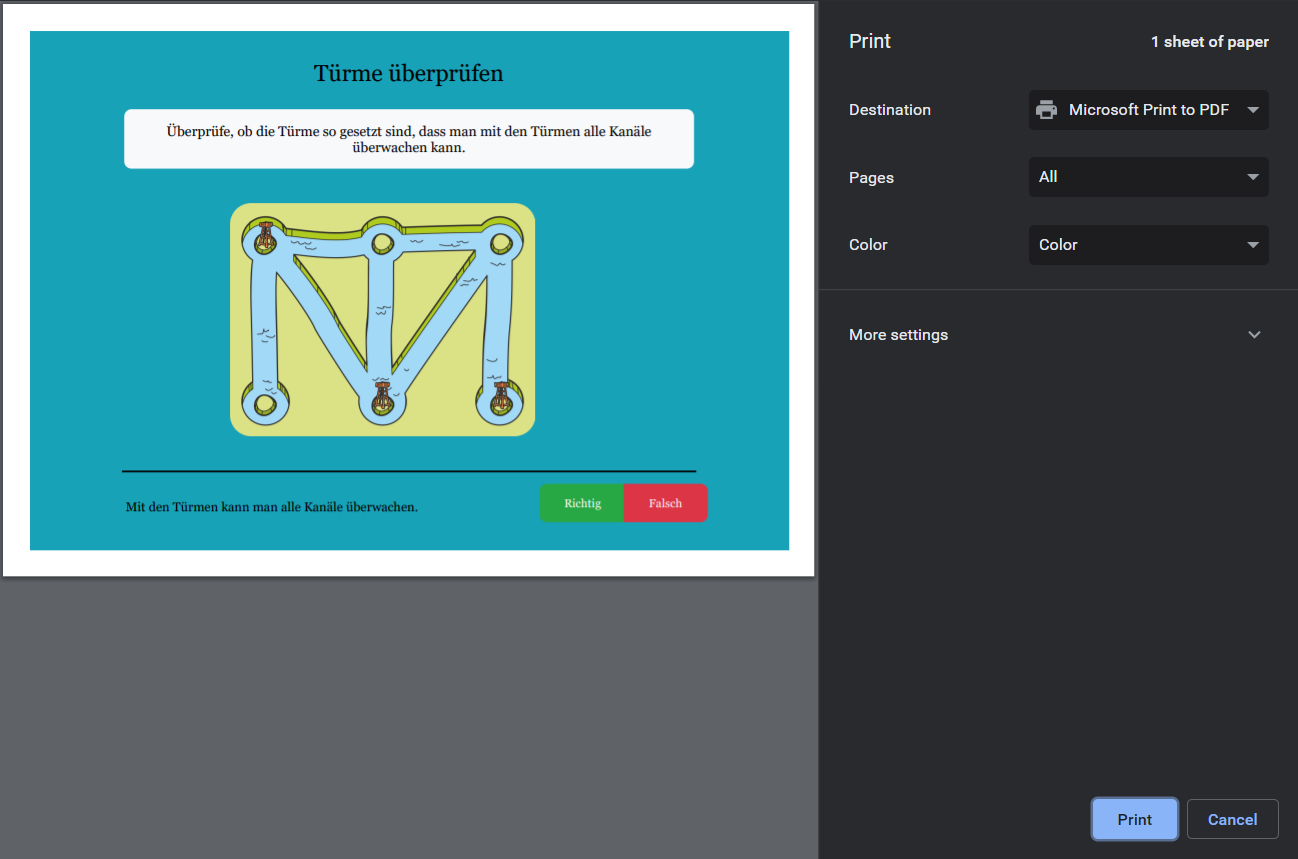
\includegraphics[width=1.0 \columnwidth]{figures/print_example.png}
    \caption{Example of a Print Window} 
    \label{fig:printex} 
\end{figure}

\subsubsection{Language Selector}
\label{subsection:language}
The language button contains the abbreviation of the language in which the environment runs momentarily. On click, the language is switched to the next available language. This button iterates through all available languages until it reaches the original language. This  is editable when one adds languages as an entry to the array 'languagePool' in the main app 'App.vue' together with a corresponding language file in the source folder in JSON format, that is named 'text\_[X].JSON', where [X] denotes a placeholder for the respective array entry of 'languagePool'. Every new language file must contain all elements and fields that the original German language file called 'text\_de.JSON' has. Otherwise, a correct functionality of the platform cannot be guaranteed.

\begin{figure}[h]
    \centering
    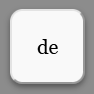
\includegraphics[width=0.15 \columnwidth]{figures/language.png}
    \caption{The Language Selector} 
    \label{fig:next} 
\end{figure}

\subsubsection{Information Button}
The information button is depicted by an encircled letter \textit{i}. It leads directly to the \nameref{subsection:about} page. This button can be found on the home screen and provides various information about the project and the learning environment.

\begin{figure}[h]
    \centering
    
\includegraphics[width=0.15 \columnwidth]{figures/about.png}
    \caption{The About Button} 
    \label{fig:next} 
\end{figure}

\subsubsection{Full Screen Button}
The button covered with a diagonal double arrow allows the user to switch from normal browser mode to full screen mode and vice versa. In full screen mode, the user experience is enhanced since all components find enough space to be properly displayed. Besides, there are no distractions when solving the tasks.

\begin{figure}[h]
    \centering
    
\includegraphics[width=0.15 \columnwidth]{figures/fullscreen.png}
    \caption{The Full Screen Button} 
    \label{fig:next} 
\end{figure}

\subsection{Routing Container}
The second main component of the page layout is the routing container. Depending on the current URL and choices made by the user, this component renders and displays different pages, in technical terms 'views'. Views correspond to different pages of the website. In the following section, views will be examined more closely. 

To enable routing to a new page, the programmer has to add the new page to a file called Views.js that is located in a folder that is called Views as well. There, the link, view and component of the new page can be specified, and the new link is automatically generated in the file index.ts that can be found in the folder called routing.

\section{Views}
\label{section:views}

As mentioned before, each page that is loaded consists of a full-page component called view and the navigation bar. Informally speaking, each so-called view corresponds to a page of the website.  Hence, there exists a view for the start page, the about page, for each game, et cetera. A view defines the build-up and layout of a page. It also specifies, which components are to be injected when rendering the page.

In the following, some particular views are presented. This will help to understand the general structure of the program.

\subsection{Home View}
The home page is the starting point whenever someone visits the website. It consists of an introductory section and a task-selector. The former gives a quick introduction to the online environment  (see figure \ref{fig:homescreen}). The latter presents the different task sets with all its levels. Each game is displayed in a box with description and a corresponding image.

\begin{figure}[H]
    \centering
    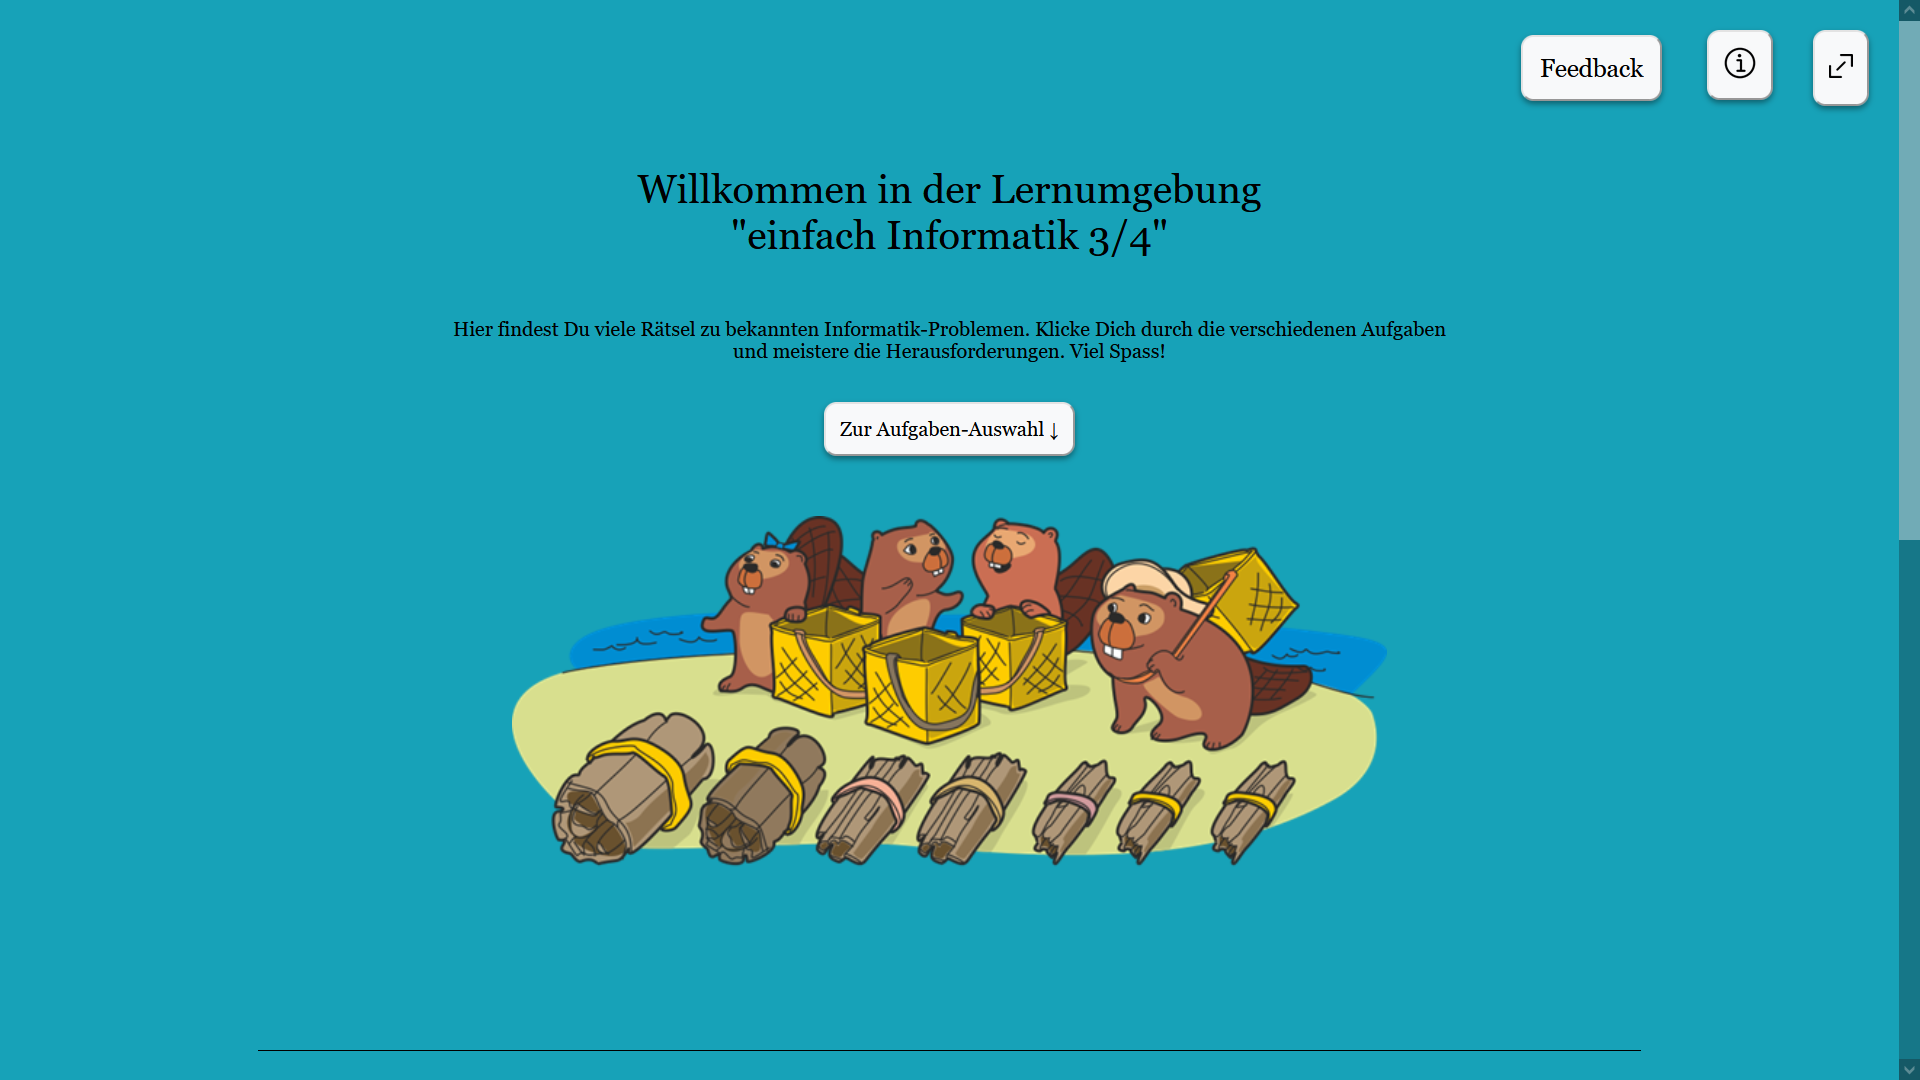
\includegraphics[width=1.0 \columnwidth]{figures/homescreen.png}
    \caption{The Home Screen} 
    \label{fig:homescreen} 
\end{figure}

\subsubsection{Task Selector}
The task selector gives an overview of all available tasks. For each game, there is a  box with the task title and a corresponding image (see figure \ref{fig:tasks}).

This container automatically lists all games that are part of the JSON file called text\_de.JSON or the file corresponding to the selected language. Any game that has been implemented and has a correct working link to access it can be added to this outline by adding it to the game section in the aforementioned JSON file.

\begin{figure}[H]
    \centering
    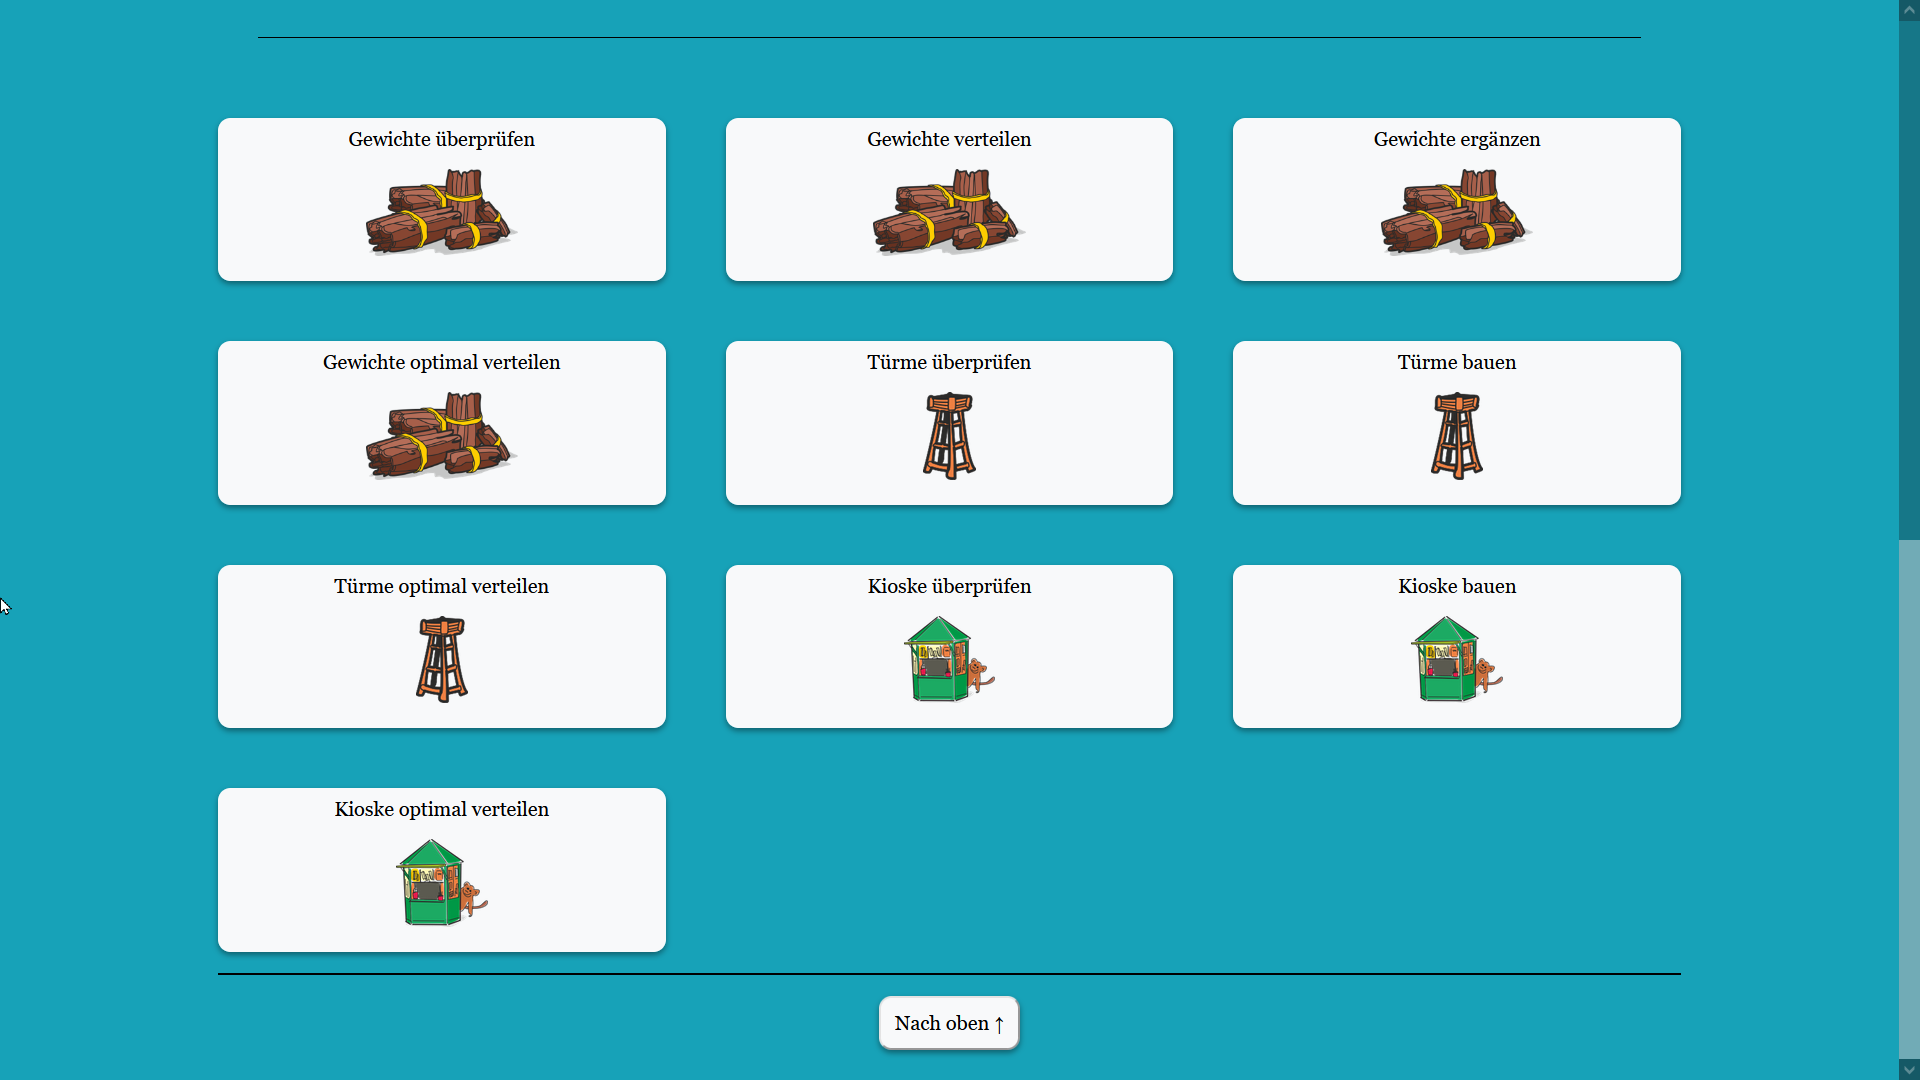
\includegraphics[width=1.0 \columnwidth]{figures/tasks.png}
    \caption{The Task Selector} 
    \label{fig:tasks} 
\end{figure}

\subsection{About View}
\label{subsection:about}
This view contains - like every other about page - all relevant information about the learning environment (see figure \ref{fig:aboutview}). Here, one can find the version, on which the platform is running. It can be useful to know what the newest features are and if the program has been updated recently. Further, information about the author and licences is provided.

\begin{figure}[H]
    \centering
    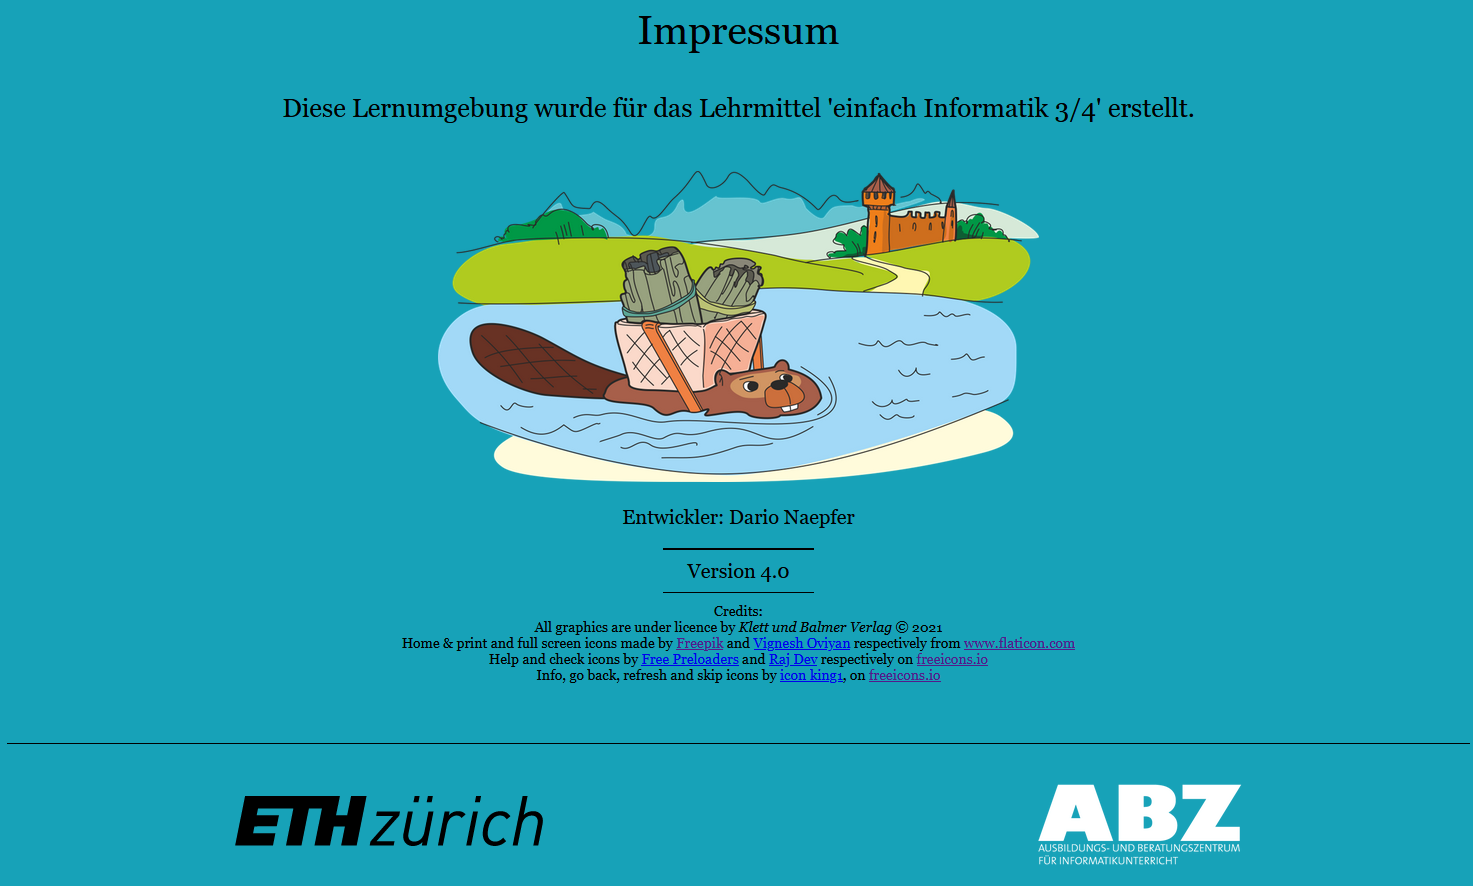
\includegraphics[width=1.0 \columnwidth]{figures/about_view.png}
    \caption{The About View} 
    \label{fig:aboutview} 
\end{figure}

\section{Game Component}
\label{section:game}

\subsection{Introduction}
The game component is the heart of the learning environment. The game component defines the general structure of the individual tasks. In this container, the game and all its features are displayed. On top of the page, there is a title referring to the actual task. The task is then introduced by an instruction sentence describing the exercise. This short introduction aims to give the user an intuition of how the task works. For more detailed explanations, one can open the instruction page for the task (see section on \nameref{subsubsection:tutorial}).

\subsection{Button Bar}
\label{subsection:buttonbar}
On the left-hand side of the game page, a button menu is displayed providing quick in-game functions. The buttons consist of symbols that give an intuition of the function they provide. When hovering over a button, the button floats to the right, and an additional description is displayed; otherwise, the text is hidden. In this way, the button menu is not too spacious and still clearly indicates its functions. There are four buttons in the following top-down order:

\subsubsection{Next Button}
The next button is represented by a right arrow. When clicked, either a new game is randomly generated or the game component is reloaded with a new map, depending on the current task. This button also resets all current game states such that a completely new task is initialized. 

\begin{figure}[H]
    \centering
    
\includegraphics[width=0.2 \columnwidth]{figures/next.png}
    \caption{The Next Button} 
    \label{fig:next} 
\end{figure}

\subsubsection{Reset Button}
The reset button is symbolized by a circular arrow. On click, a function is called that completely resets the current game state such that the current game can be played again from its initial position. Clicking this button does only affect the recent user inputs concerning the actual task.

\begin{figure}[H]
    \centering
    
\includegraphics[width=0.2 \columnwidth]{figures/restart.png}
    \caption{The Reset Button} 
    \label{fig:next} 
\end{figure}

\subsubsection{Verify Button}
The tick surrounded by a circle depicts the check button that can be called whenever an input should be verified. When the button is clicked, a pop-up window opens giving individual feedback on how well the task has been solved, including a beaver (see figure \ref{fig:beavers}). The user input is evaluated as either correct or incorrect. On a correct input, the modal window shows a celebrating beaver indicating that the task has been successfully completed. If this is not the case, a disappointed beaver is displayed coupled with a feedback or tip depending on the improvements that ought to be made. The user is advised to either first comply with the instructions or rethink the provided solutions.

\begin{figure}[H]
    \centering
    
\includegraphics[width=0.2 \columnwidth]{figures/check.png}
    \caption{The Verify Button} 
    \label{fig:next} 
\end{figure}

\begin{figure}[H]
    \centering
    
\includegraphics[width=0.7 \columnwidth]{figures/evaluation_result.png}
    \caption{The two beavers indicating the result correctness} 
    \label{fig:beavers}
\end{figure}

\subsubsection{Tutorial}
\label{subsubsection:tutorial}
The encircled question mark represents the tutorial button. By clicking it, one can find a more detailed description of the current task. The tutorial opens up in an overlay window that consists of a title, an extensive description as well as a tutorial video, individually created for each task or task set. An example is provided in the figure below.

\begin{figure}[H]
    \centering
    
\includegraphics[width=0.2 \columnwidth]{figures/tutorial.png}
    \caption{The Tutorial Button} 
    \label{fig:tutorial} 
\end{figure}

\begin{figure}[H]
    \centering
    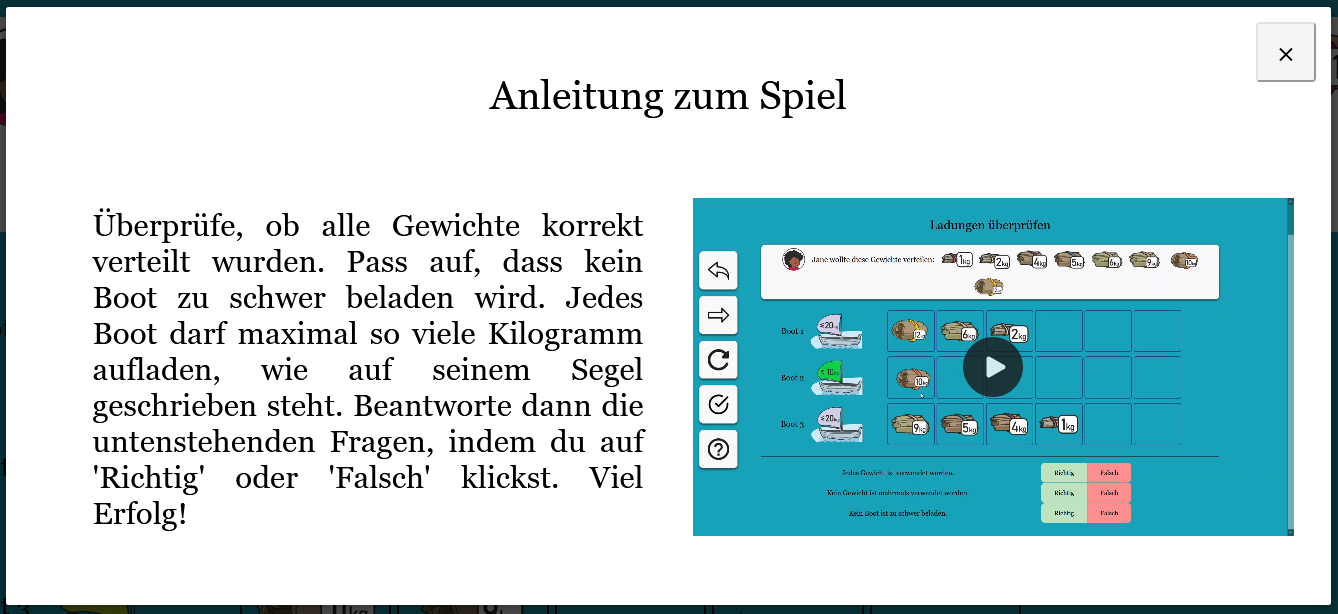
\includegraphics[width=1 \columnwidth]{figures/tutorial_example.png}
    \caption{Example of a Task Tutorial} 
    \label{fig:next} 
\end{figure}

\subsection{Difficulty Switch}
In one of the tasks, one can also find a difficulty switch in this section. On click, the difficulty is toggled between a lower difficulty level illustrated by a single standing beaver and a higher difficulty level depicted by two beavers. Whenever the button is clicked, the game is completely restarted and a new game instance is created.

\begin{figure}[H]
    \centering
    
\includegraphics[width=0.4 \columnwidth]{figures/levels.png}
    \caption{The Difficulty Switch} 
    \label{fig:levels} 
\end{figure}

\newpage
\subsection{Statement Check}
\label{subsection:statementcheck}
In each of the three task types, there is a difficulty level where suggested solutions for the task have to be reviewed by the user. Hence, a reusable component was created for this purpose. It can be integrated in each of the task templates. This component automatically generates a statement including a true/false button for each string that is passed as an argument. True and false can be toggled by clicking on the statement itself or on the corresponding button. The parameter called statements is an array with tuples consisting of a number and a statement. The array can contain any number of tuples and will create a proposition for each string.

\begin{figure}[H]
    \centering
    
\includegraphics[width=0.3 \columnwidth]{figures/tf-buttons.png}
    \caption{The Statement Check Buttons} 
    \label{fig:statement} 
\end{figure}
